\documentclass{ximera}

\title{Tutorial}

\begin{document}
\begin{abstract}
  This course is built in Ximera.
\end{abstract}\maketitle

Mathematics cannot be learned passively: it must be actively
\href{http://en.wikipedia.org/wiki/Constructivism_(philosophy_of_education)}{constructed}
by the person learning it.  With this in mind, this course
is built around solving problems!

Here is an example problem.  Play around with it, get it wrong, try
the hints out.  Don't be afraid to fail: getting an answer wrong never
hurts you.

\begin{question}
    $3\times 2 = $ \answer{6}
   
    \begin{hint}
      $3 \times 2$ is the number of objects in $3$ groups of $2$ objects
    \end{hint}
    \begin{hint}
      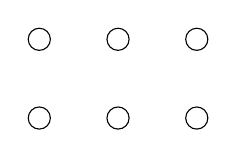
\begin{tikzpicture}
        \draw (0,0) circle (4pt);
        \draw (1,0) circle (4pt);
        \draw (2,0) circle (4pt);
        \draw (0,1) circle (4pt);
        \draw (1,1) circle (4pt);
        \draw (2,1) circle (4pt);
      \end{tikzpicture}
    \end{hint}
    \begin{hint}
      $3\times 2=6$
    \end{hint}
\end{question}

For this course, you should always have a paper and pencil near at hand to make notes, doodle pictures, or solve complicated equations.
We \textbf{strongly} recommend that you really \textbf{grapple} with a problem before getting a hint, or moving on.  
The difference between what you learn by struggling with a problem on your own versus perusing someone else's solution is astonishing.

With that said, even if you get an answer right you should \textbf{always} try the
hints out afterwards.  They might explain the concept from a new point
of view, or challenge you to think in a different way than you solved
the problem.
\\
\\
We support a few different answer types: as you have seen above,
numerical answers are one type.  Here are some example problems from
the different answer types we support:
\\
\\
\begin{question}

  \textbf{An expression answer type}

Try writing the expression $x^2+y$ = \answer{x^2+y}.  Try failing first, to see what happens.

    \begin{hint}
      Great!  You looked at this hint.  That is totally what you were supposed to do.
    \end{hint}

    \begin{hint}
      Sometimes hints have problems in them.  Usually these problems would be a simpler version of the question you are trying to answer, or a crucial part of the solution.  In this case, it is just a demo of problems within hints:
      

	\begin{question}

        The last sultan of the Ottoman Empire was:
	
	\begin{multipleChoice}
            \choice[correct]{Abdülmecid II}
            \choice{Abdülhamid II}
            \choice{Suleiman II}
	\end{multipleChoice}

          \begin{hint}
            Check Wikipedia!
          \end{hint}

          \begin{hint}
            The correct answer is Abdülmecid II.
          \end{hint}

 	\end{question}

    \end{hint}

\end{question}

\begin{question}
  \textbf{Multiple choice and multiple select}


	\begin{question}
	Which single answer is correct?
	\begin{multipleChoice}
		\choice[correct]{This one!}
		\choice{Not this}
		\choice{Not this either}
		\choice{Also not this}
	\end{multipleChoice}
	\end{question}

	\begin{question}
	Which of the following answers are correct?
	\begin{selectAll}
		\choice[correct]{This one!}
		\choice{Not this}
		\choice[correct]{This one too!}
		\choice{Also not this}
	\end{selectAll}
	\end{question}
	
\end{question}

A free response answer type:

Tell us who you are and why you are taking this course!

\begin{freeResponse}
We are the mysterious authors...
\end{freeResponse}


As you complete activities the green ``completion bar''  moves at
the top of the page.  This lets you know how close you are to being
done with an activity.

You advance through pages either by completing them and clicking the
``next activity'' button, or by navigating on the little scroll bar at the top of the page.
 
Only one more question left:
\begin{question}
    Are you ready to start learning some Calculus!?!
    
    \begin{multipleChoice}
      \choice[correct]{Yes I am!}
    \end{multipleChoice}

      \begin{hint}
        We promise the real course will not be this corny.
      \end{hint}

\end{question}

\end{document}
